\subsection{Echo chambers}
In news media, \textit{echo chamber} is a metaphorical description of a situation in which beliefs are amplified or reinforced by communication and repetition inside a closed system \cite{echochamwiki}\cite{echocham}.\\
We qualitatively investigated the presence of echo chambers in our network.
First of all, our agents have a ``mental  state'', i.e. a vector of preferences: its components represent the amount of interest toward a certain topic.\\
 News have the same dimension of \textit{mental state vector} (MSVD) in order to establish a ``matching'' between news' topics and users' preferences. 
 Mental state is higly involved in news' dynamics and network topology: see \cite{ourpaper} for more details.
 In the images below, for MSVD=3,5,7, we extracted main clusters from our network.
 \textit{Modularity} is a measure for detecting community structure in graph\cite{modulwiki}.
 Nodes were painted with modularity class and belonging news for a comparison: in case of news' homogeneity inside a single cluster, we are observing an echo chamber.
 We can notice that number of clusters equals MSVD basically.
 News' situation is more heterogenous: altough some clusters still exist, there is not a clear separation among users with different news. 
 
 
\begin{figure}

  \centering
  \begin{subfigure}[t]{0.25\textwidth}
    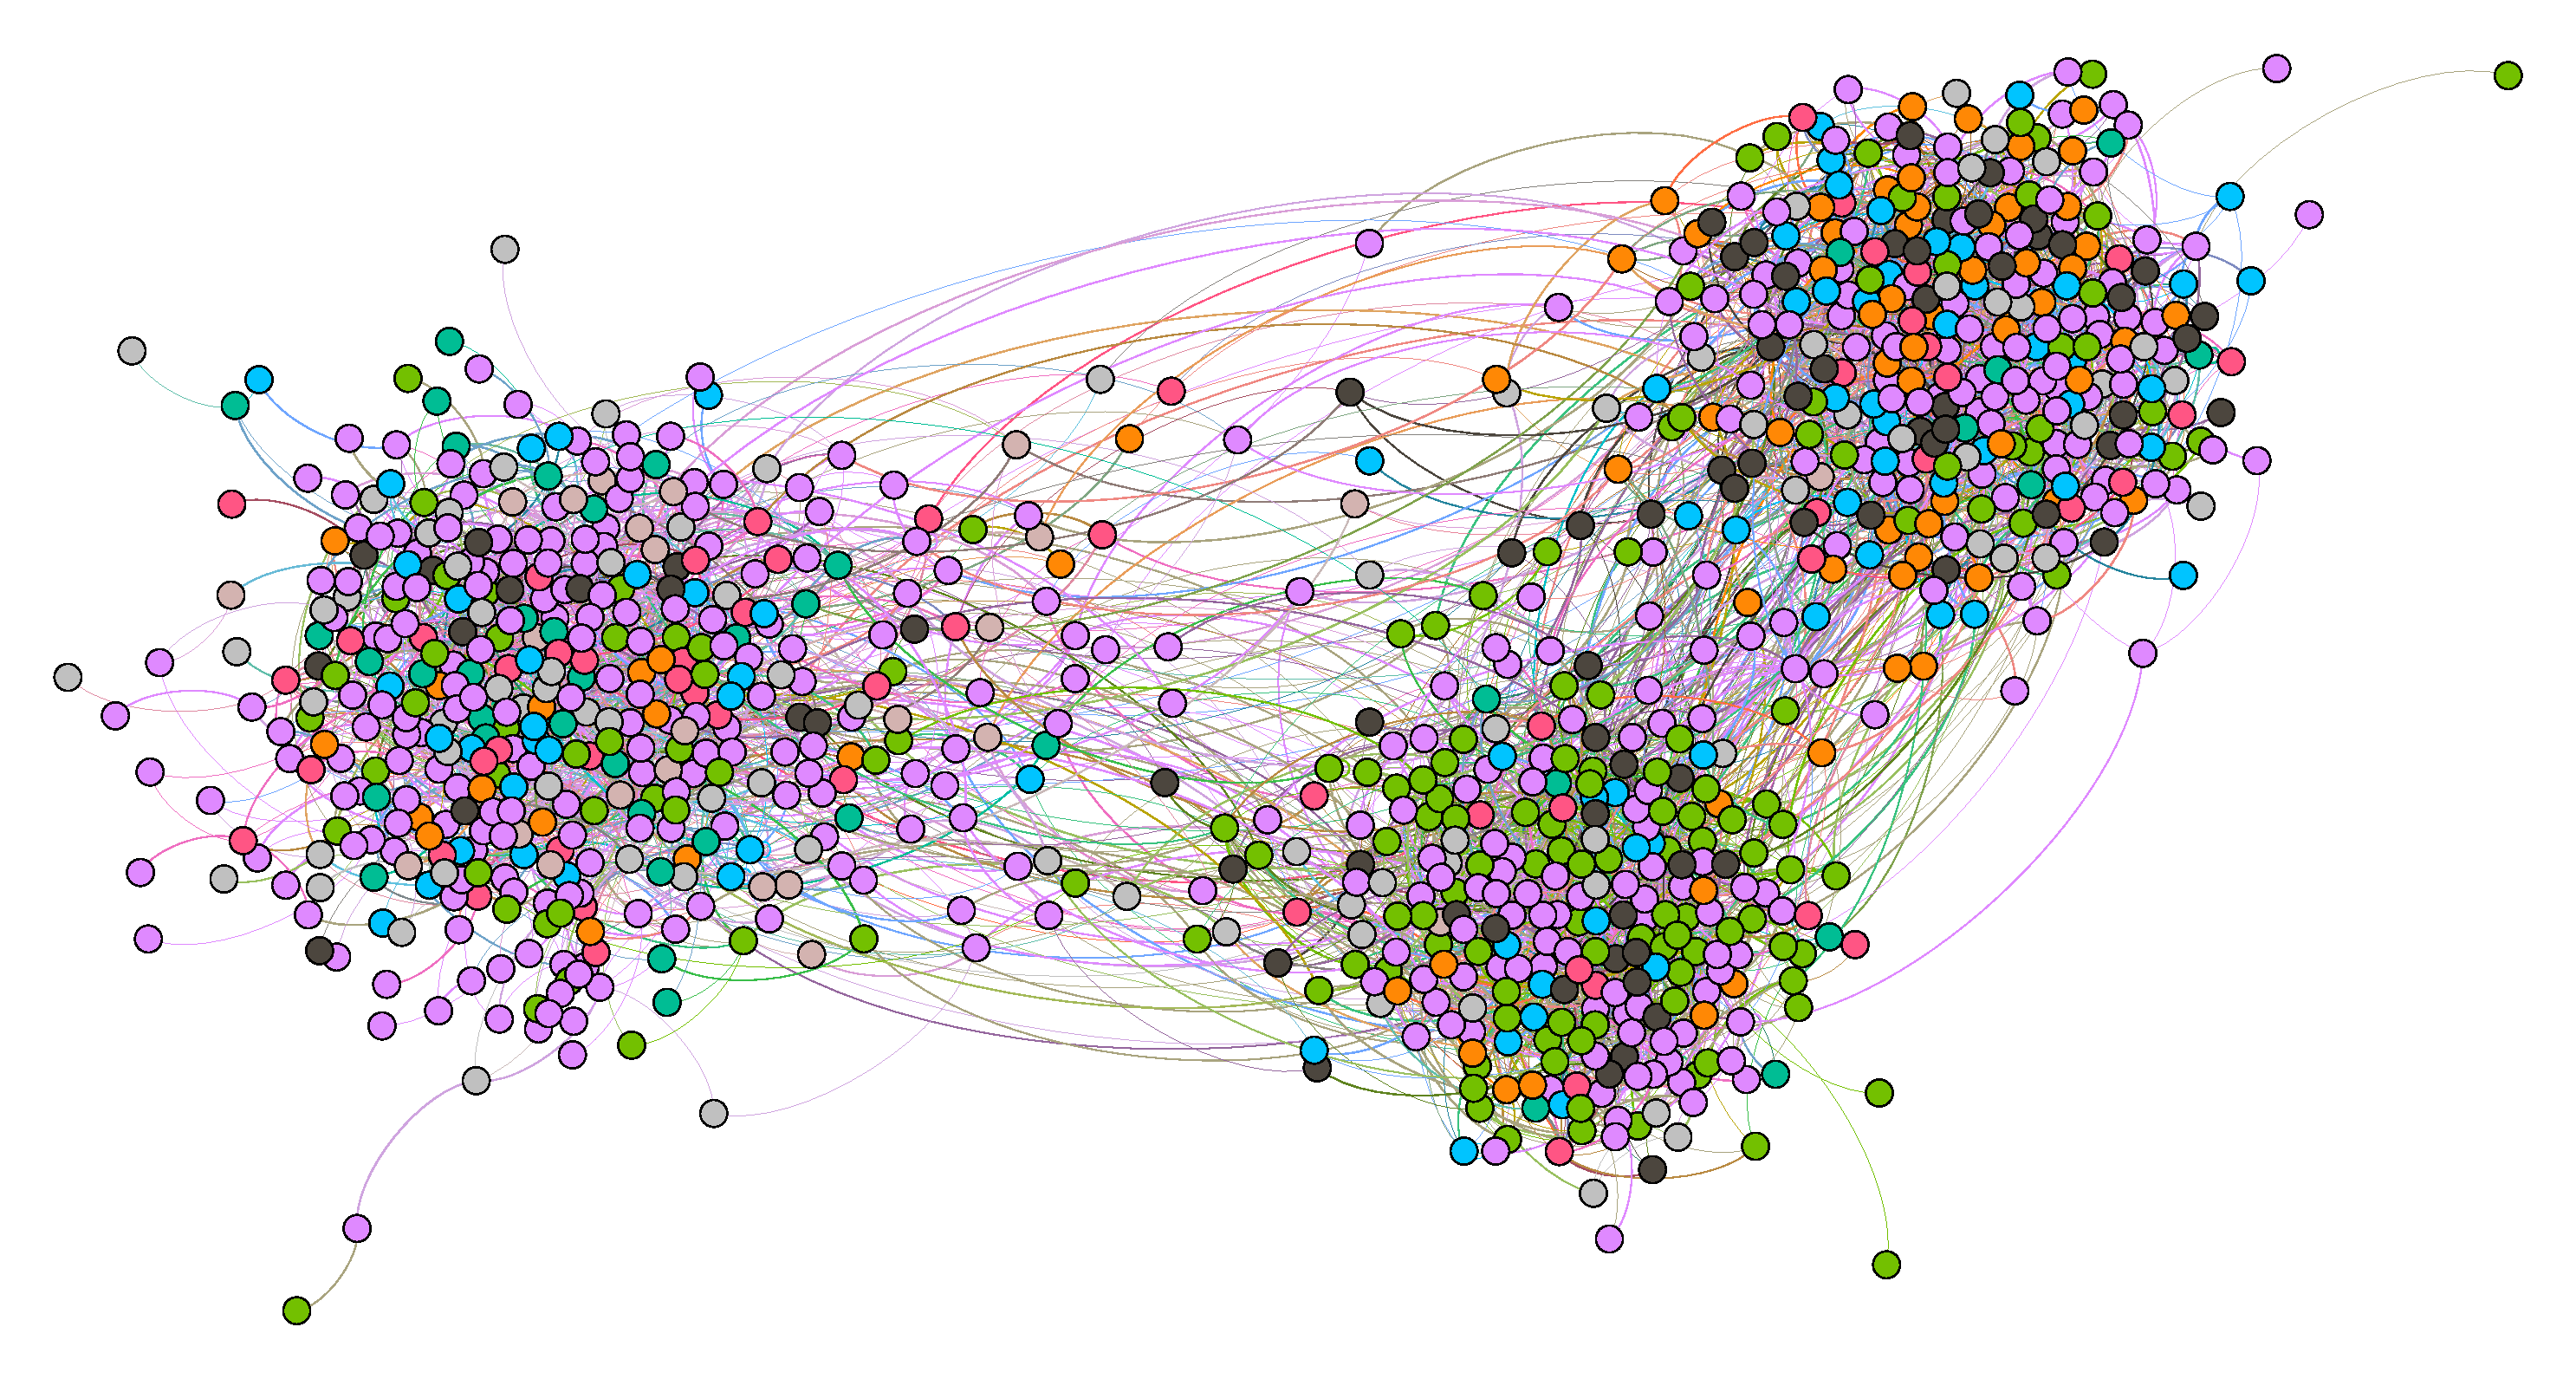
\includegraphics[width=\textwidth]{img/dim3_mod.pdf}
    \label{fig:bubble3mod}
    \caption{}
  \end{subfigure}
  ~
  \begin{subfigure}[t]{0.35\textwidth}
    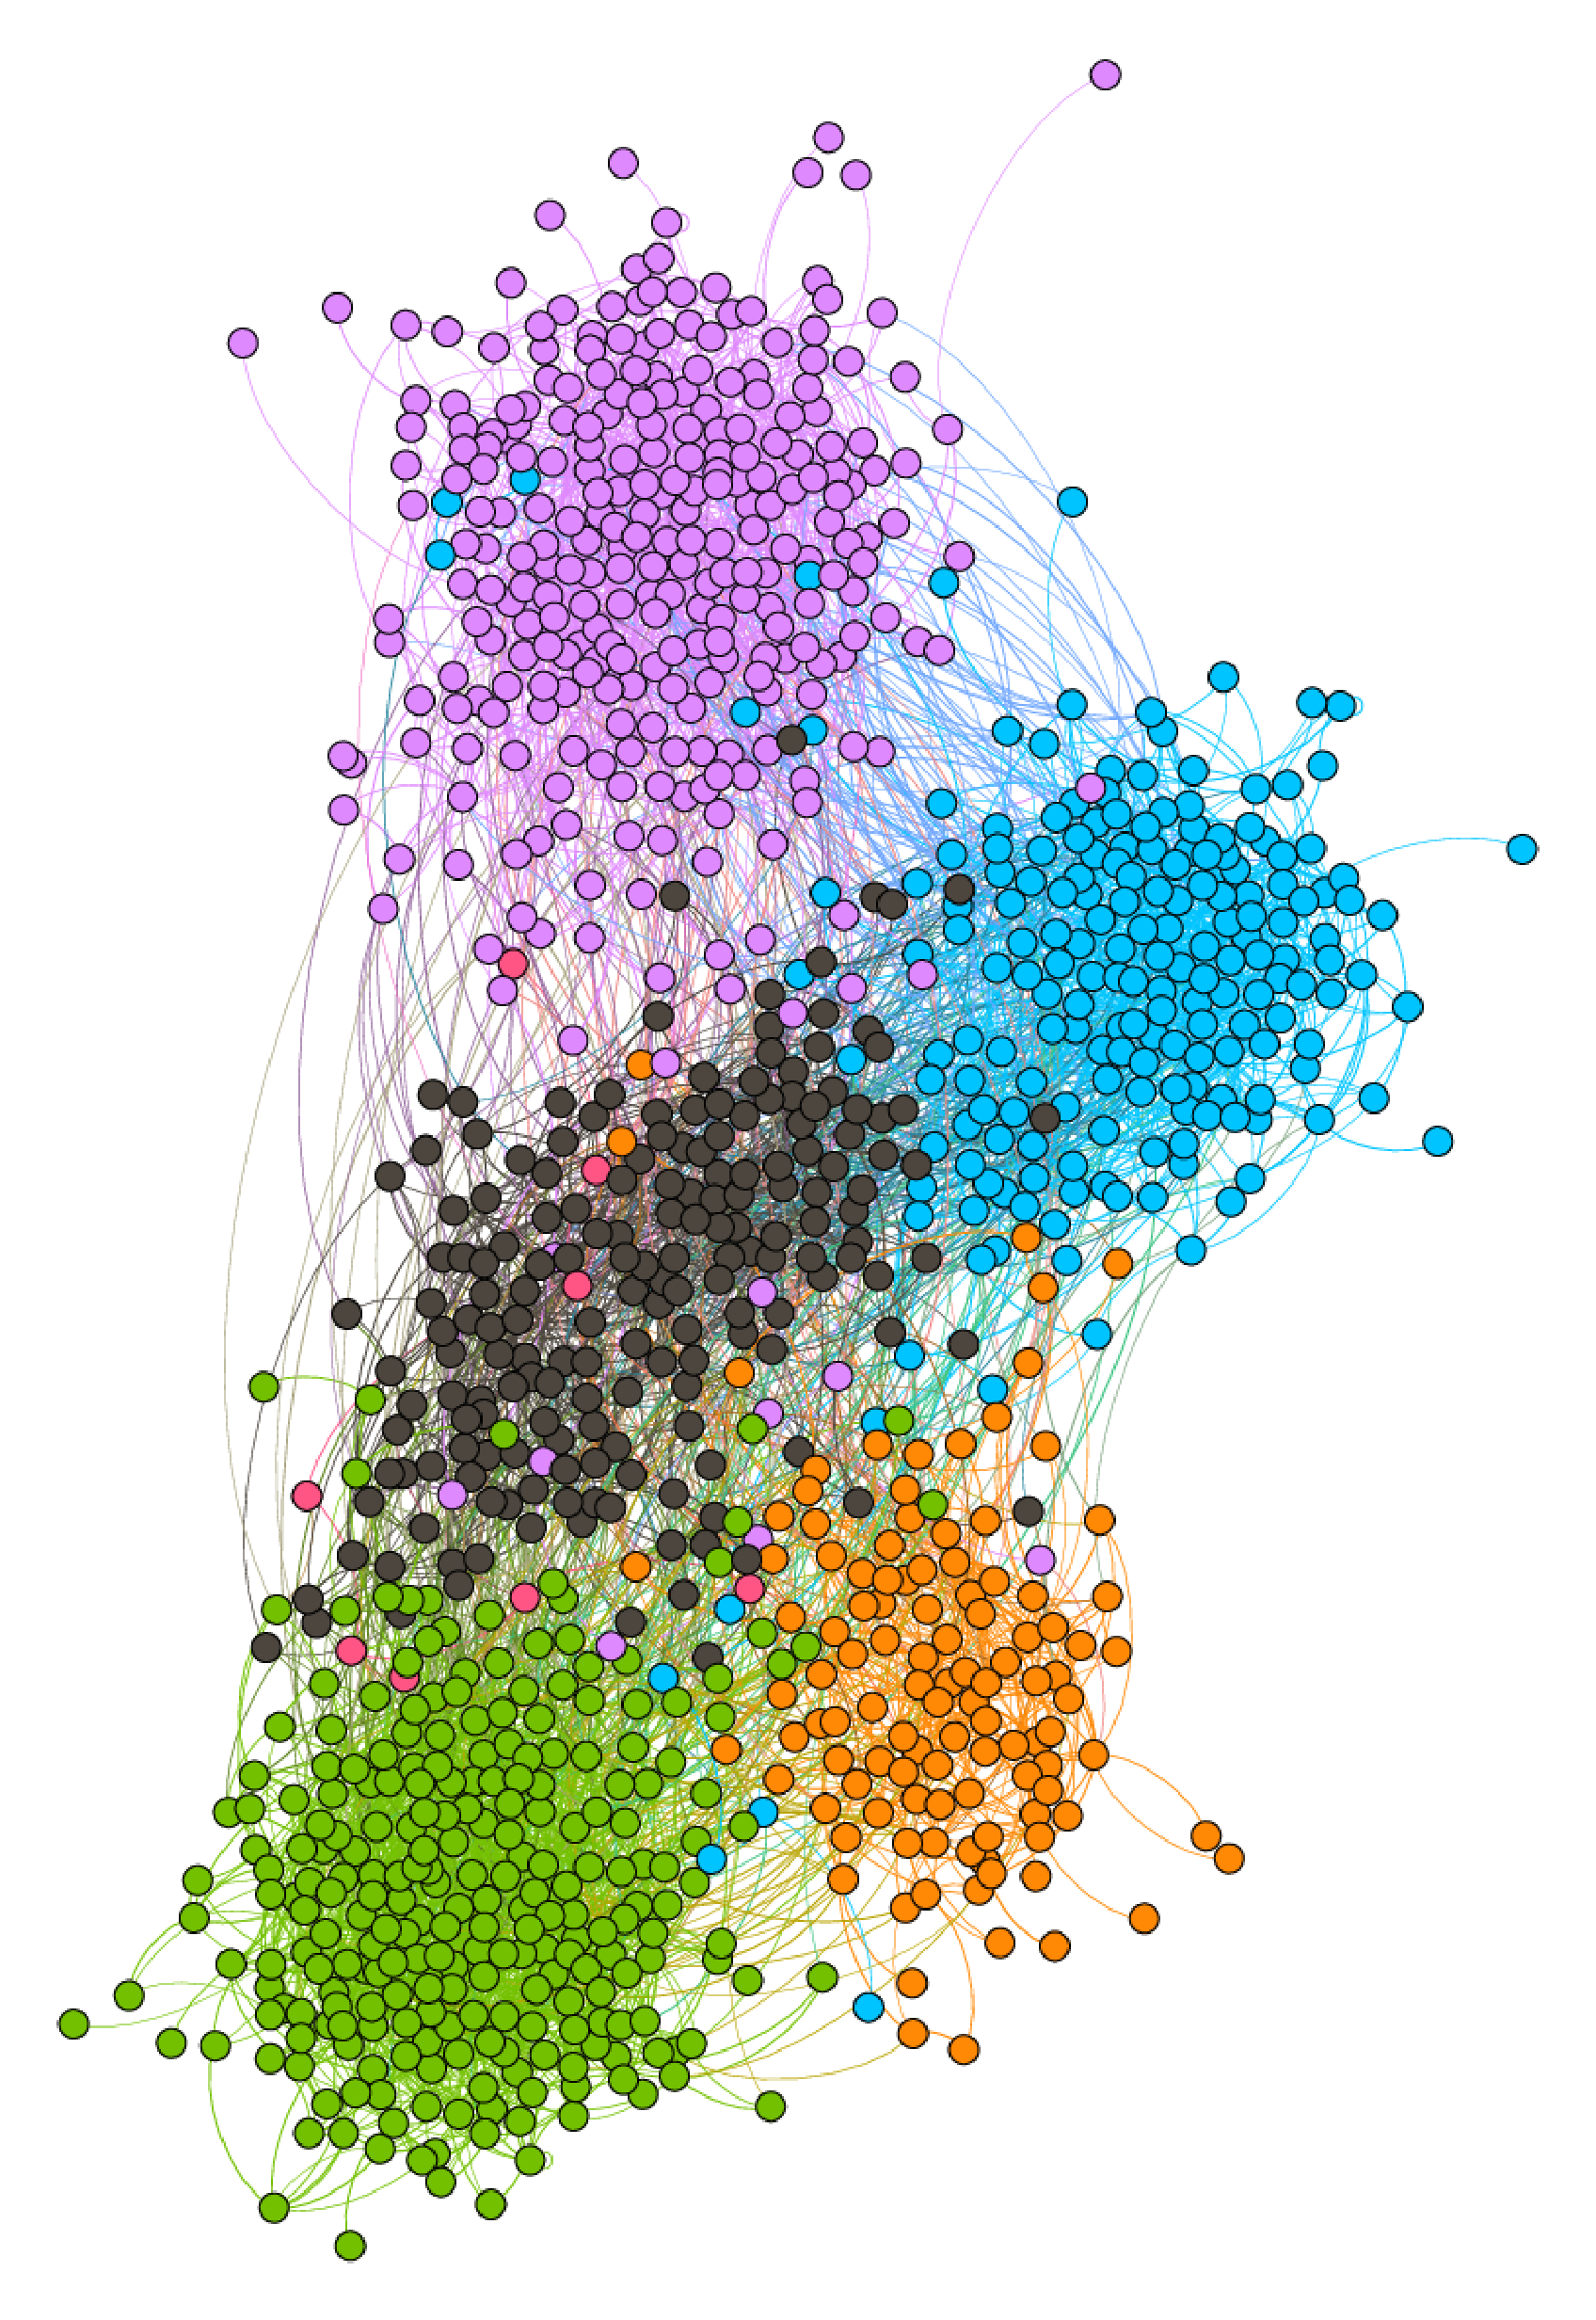
\includegraphics[width=\textwidth]{img/dim5_mod.pdf}
    \label{fig:bubble5mod}
    \caption{bubble3news}
  \end{subfigure}
  ~
  \begin{subfigure}[t]{0.35\textwidth}
    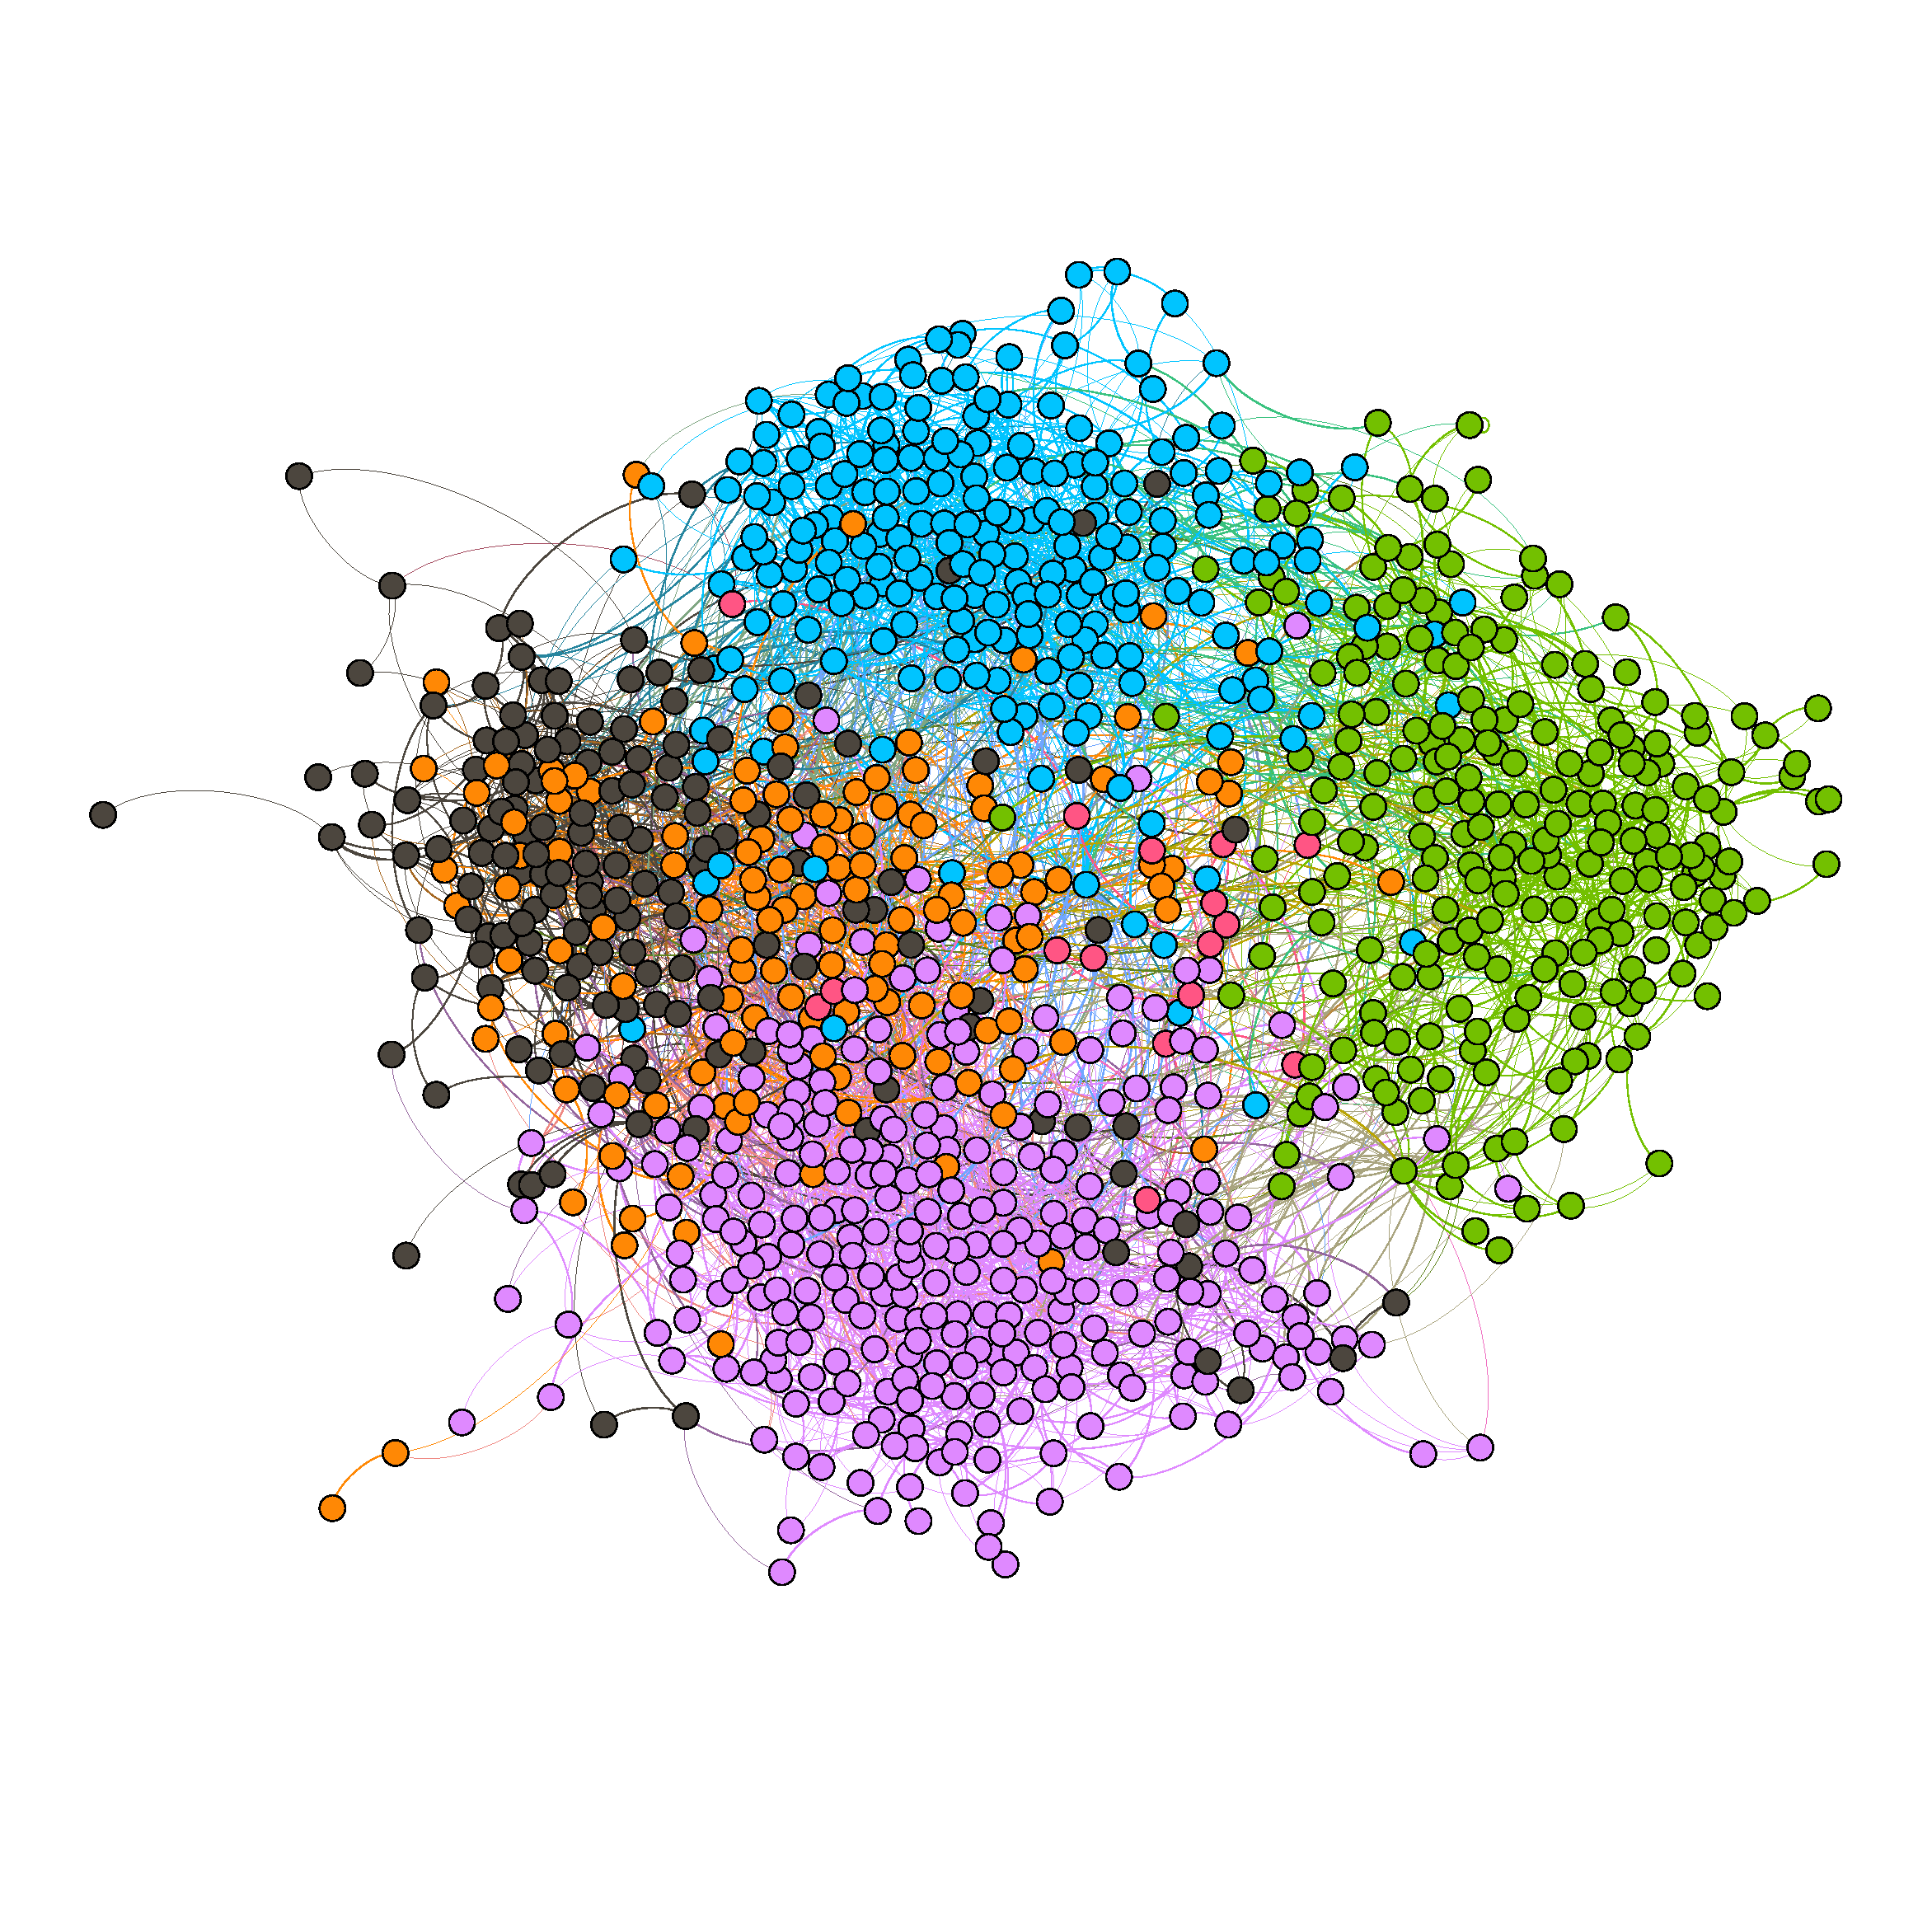
\includegraphics[width=\textwidth]{img/dim7_mod.pdf}
    \label{fig:bubble7mod}
    \caption{bubble3news}
  \end{subfigure}
  \\
  \begin{subfigure}[t]{0.25\textwidth}
    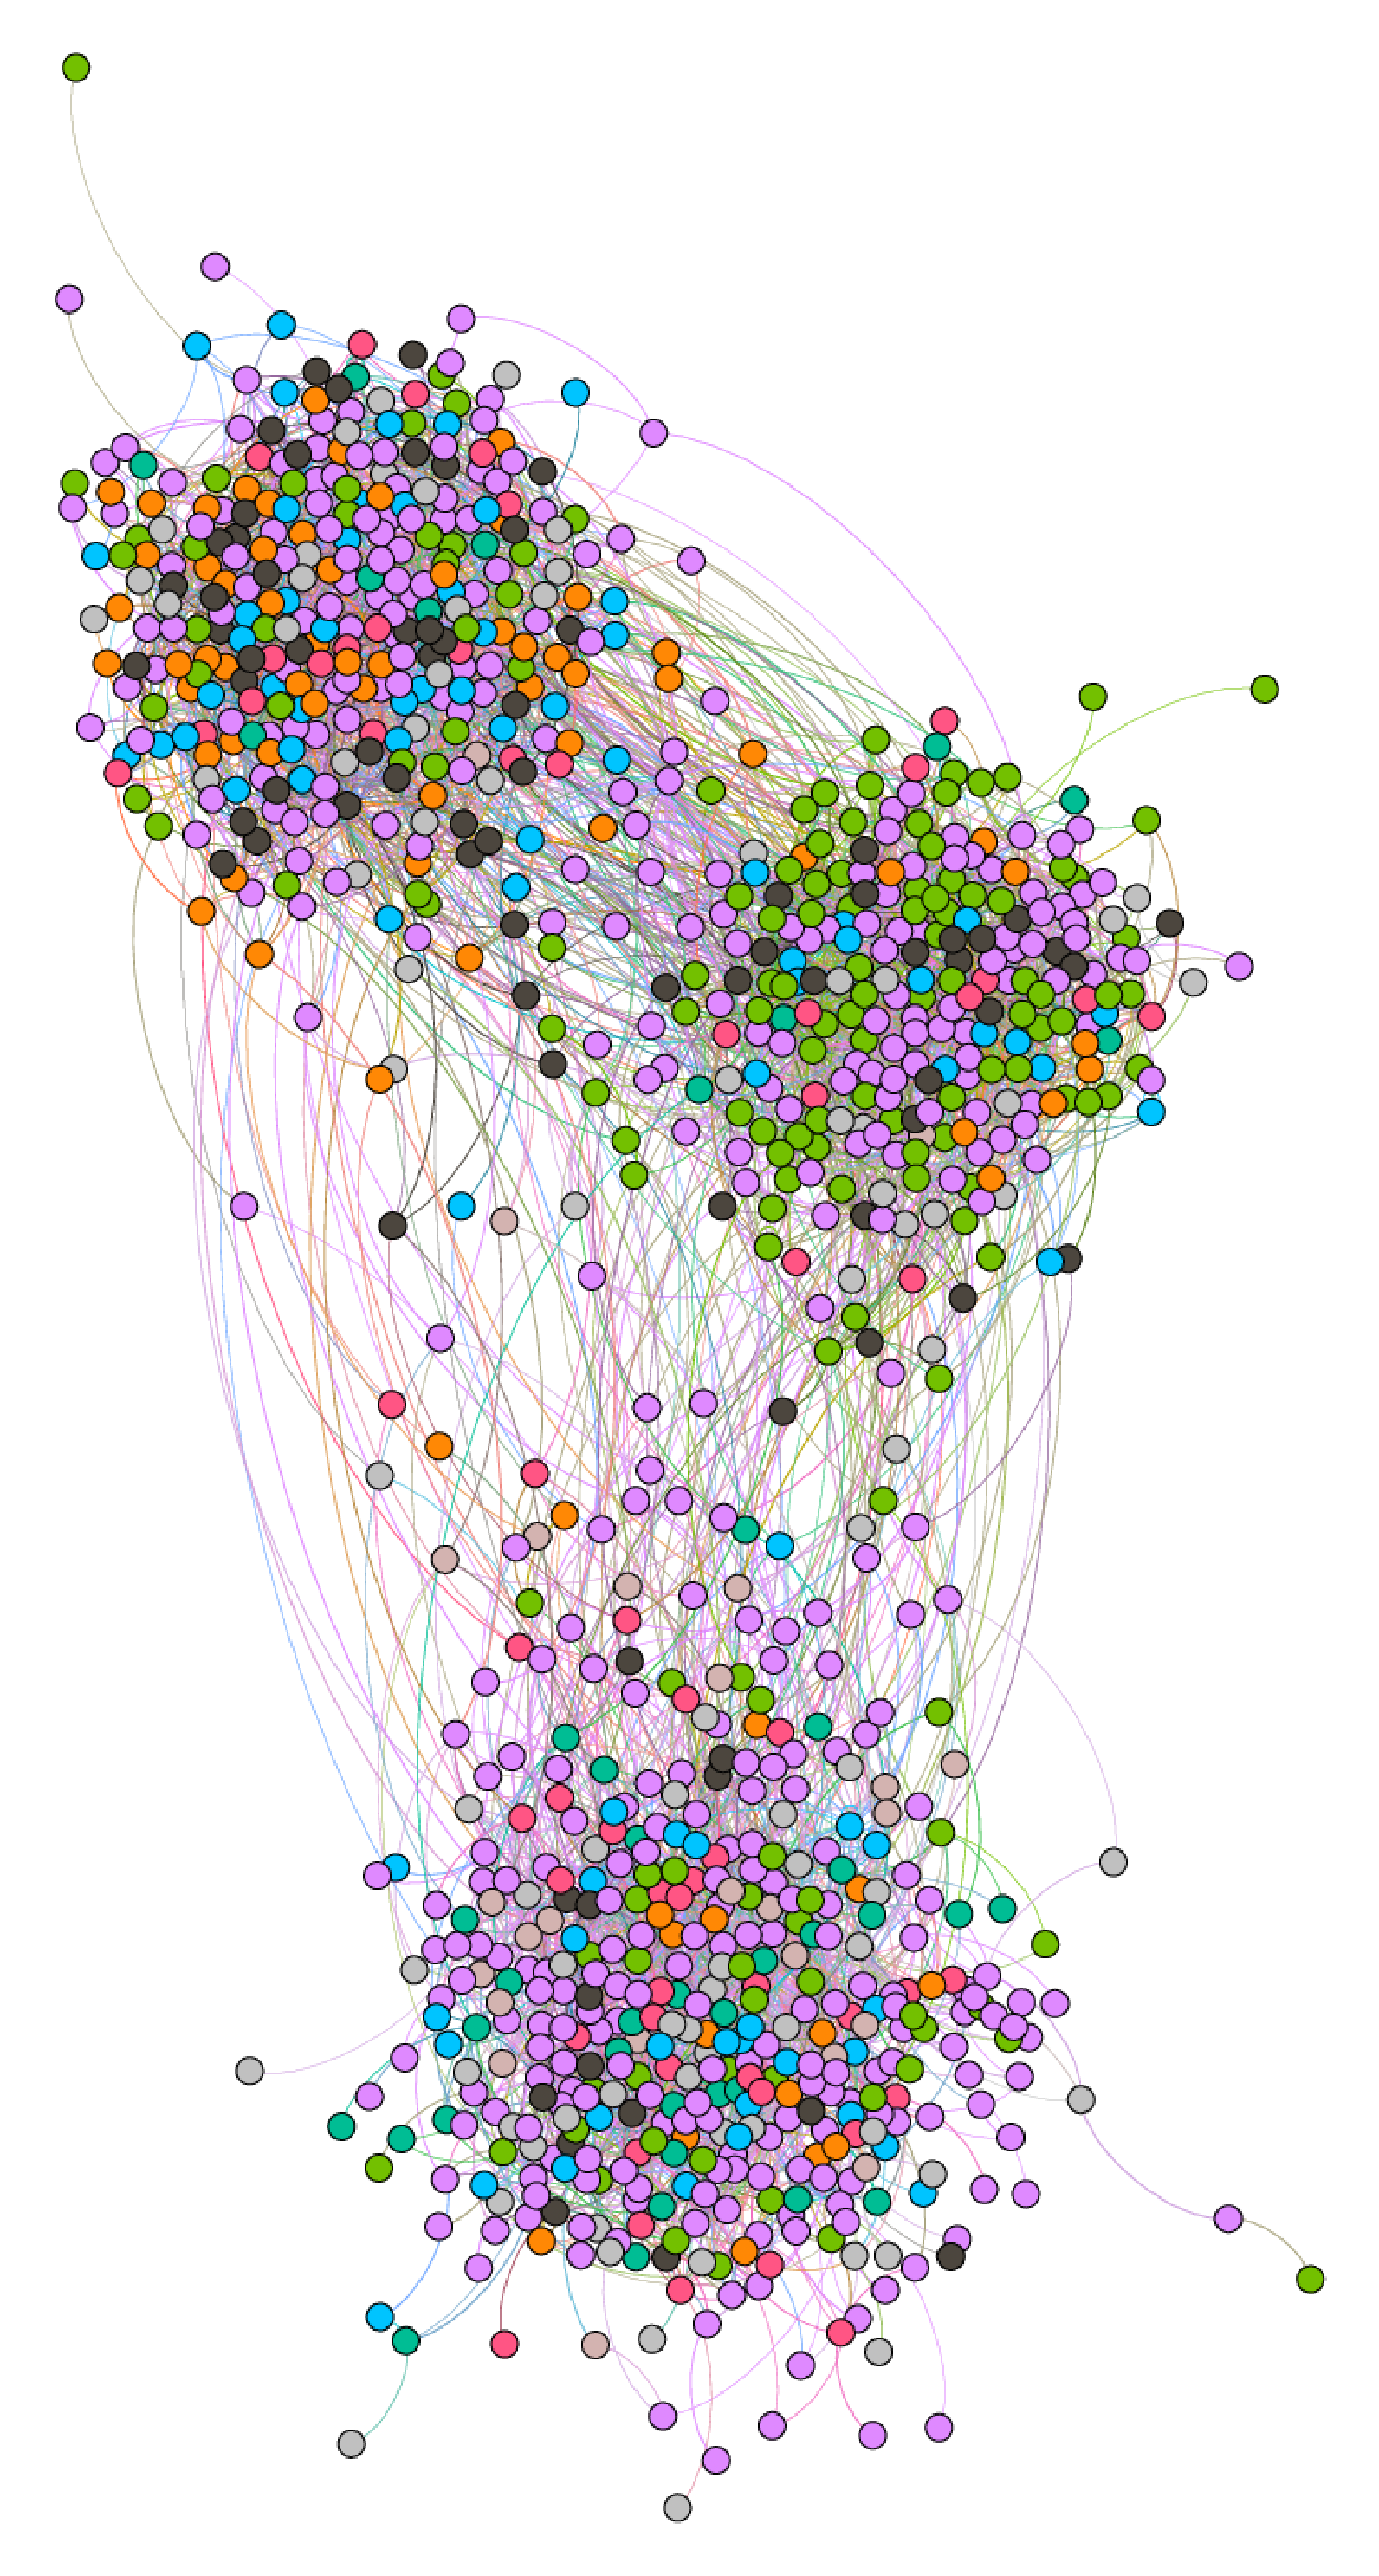
\includegraphics[width=\textwidth]{img/dim3_news.pdf}
    \label{fig:bubble3news}
    \caption{bubble3mod}
  \end{subfigure}
  ~
  \begin{subfigure}[t]{0.35\textwidth}
    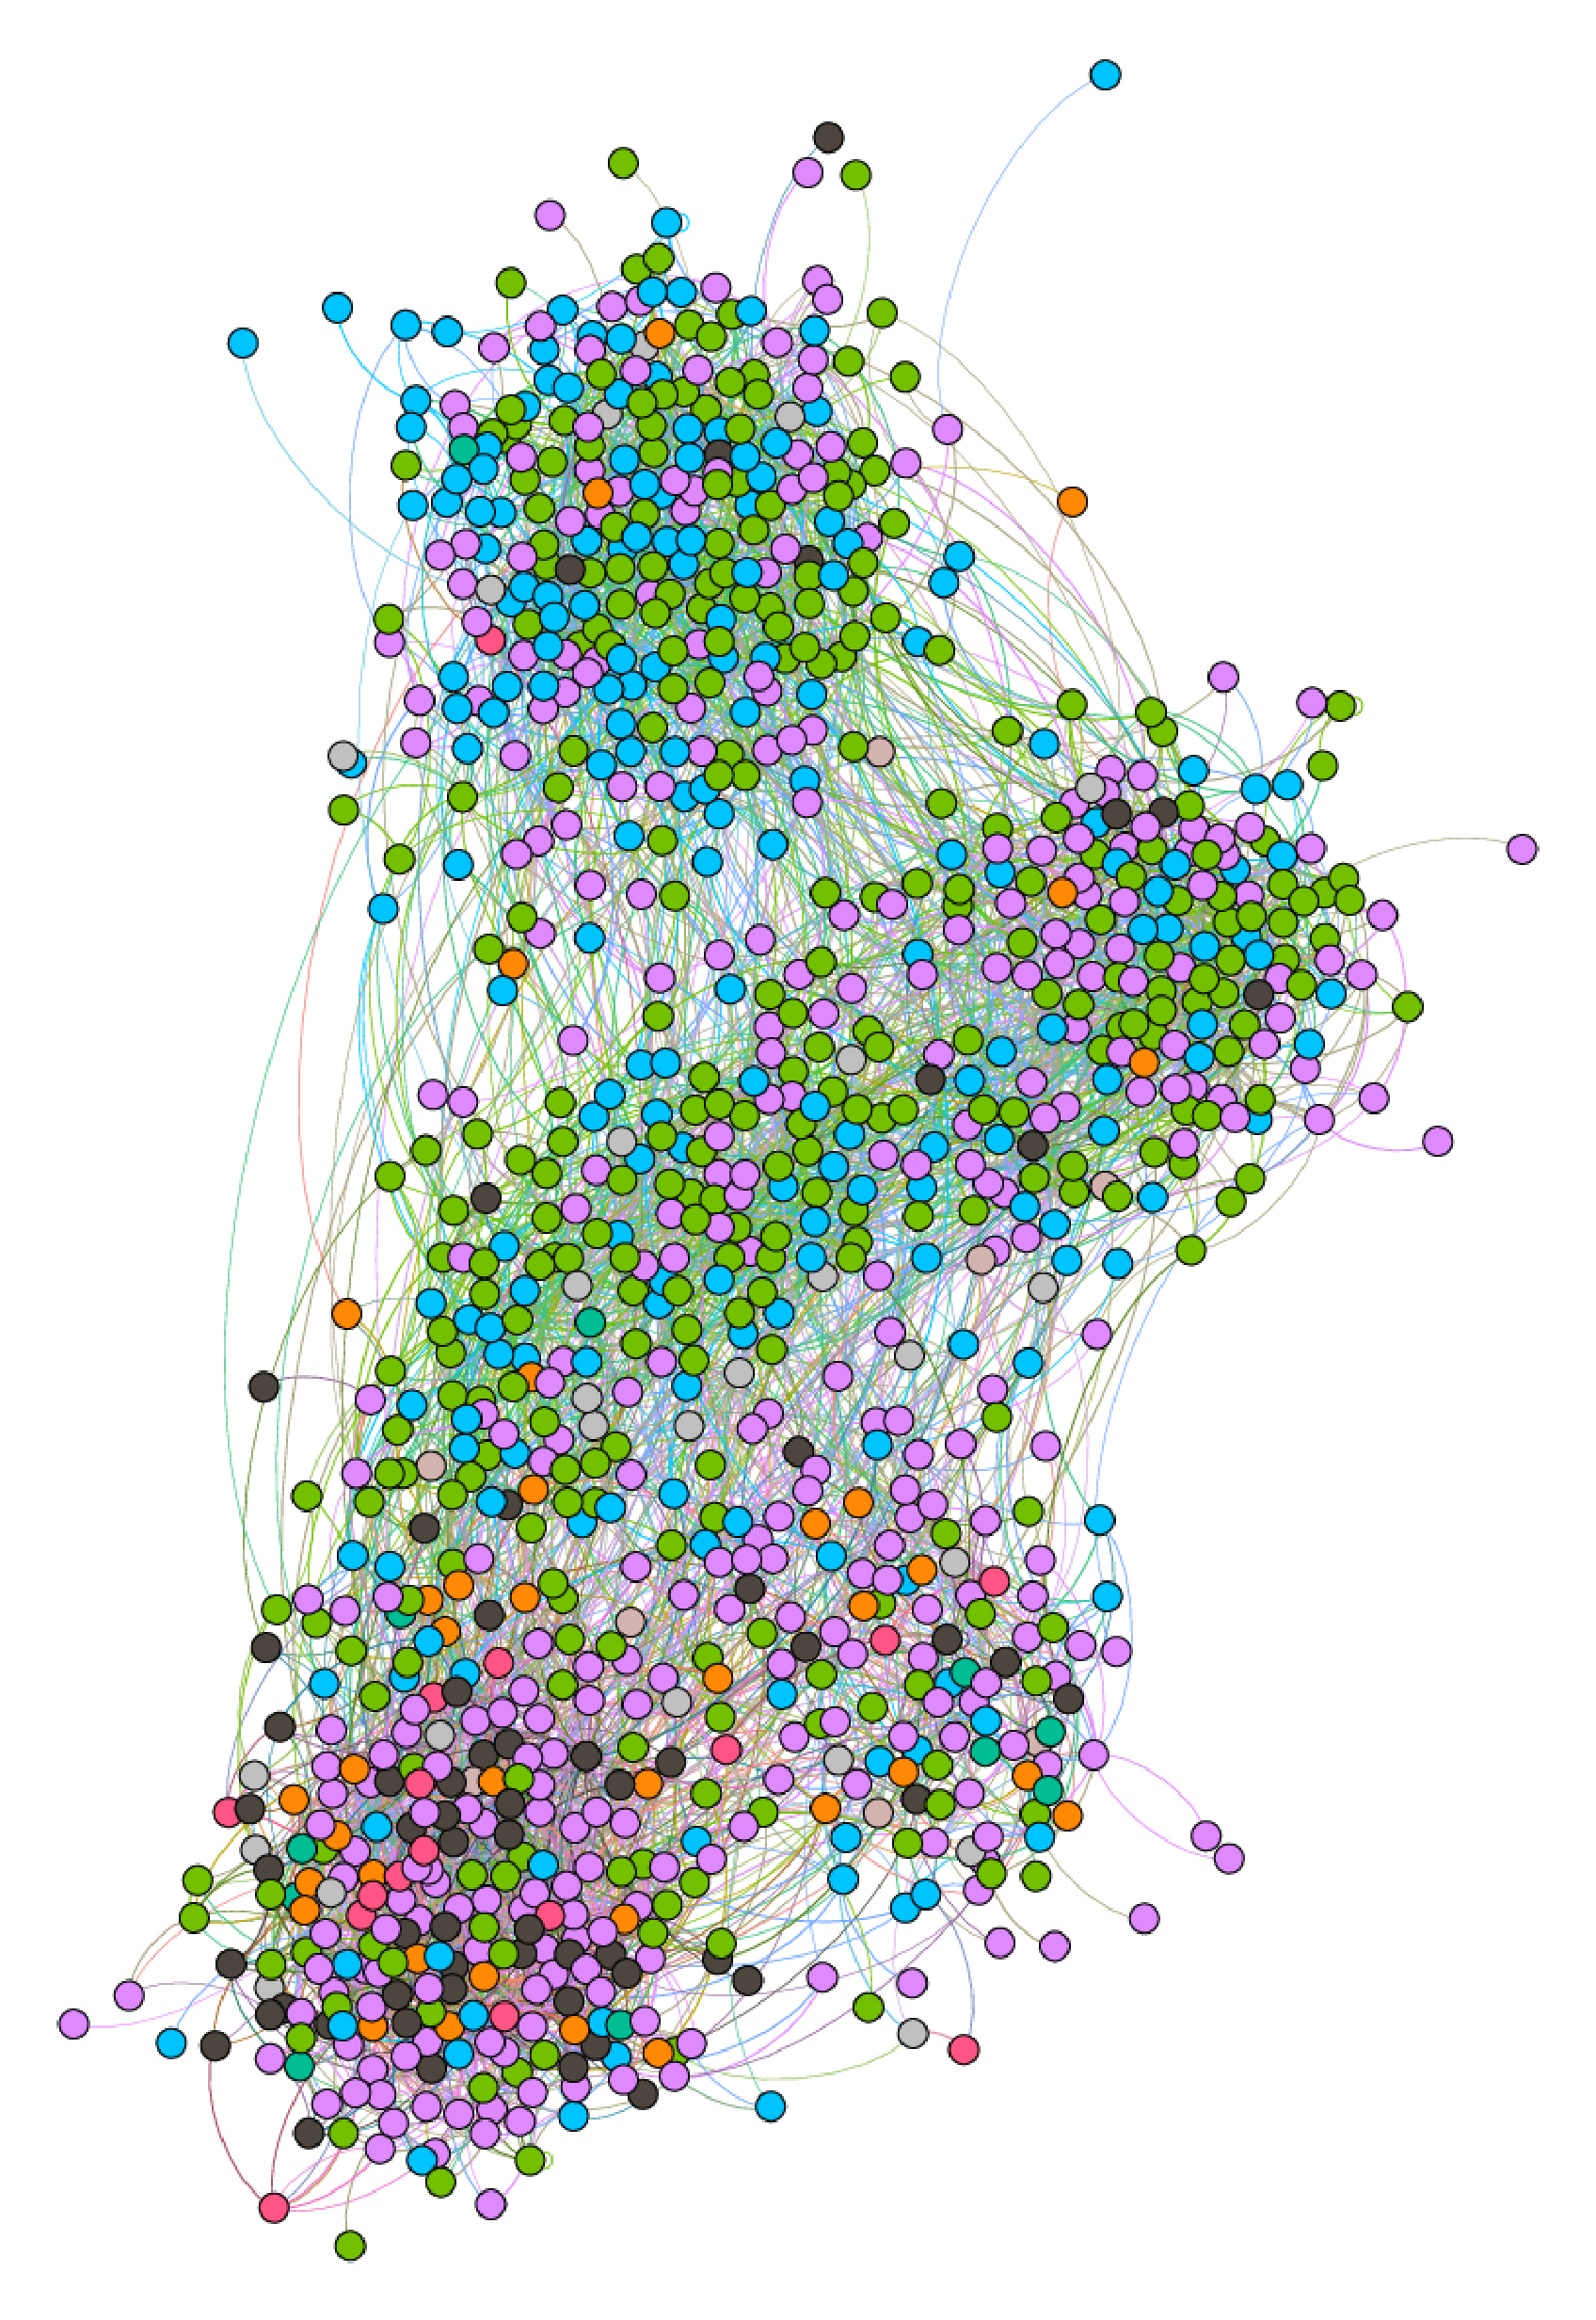
\includegraphics[width=\textwidth]{img/dim5_news.pdf}
    \label{fig:bubble5news}
    \caption{bubble3news}
  \end{subfigure}
  ~
  \begin{subfigure}[t]{0.35\textwidth}
    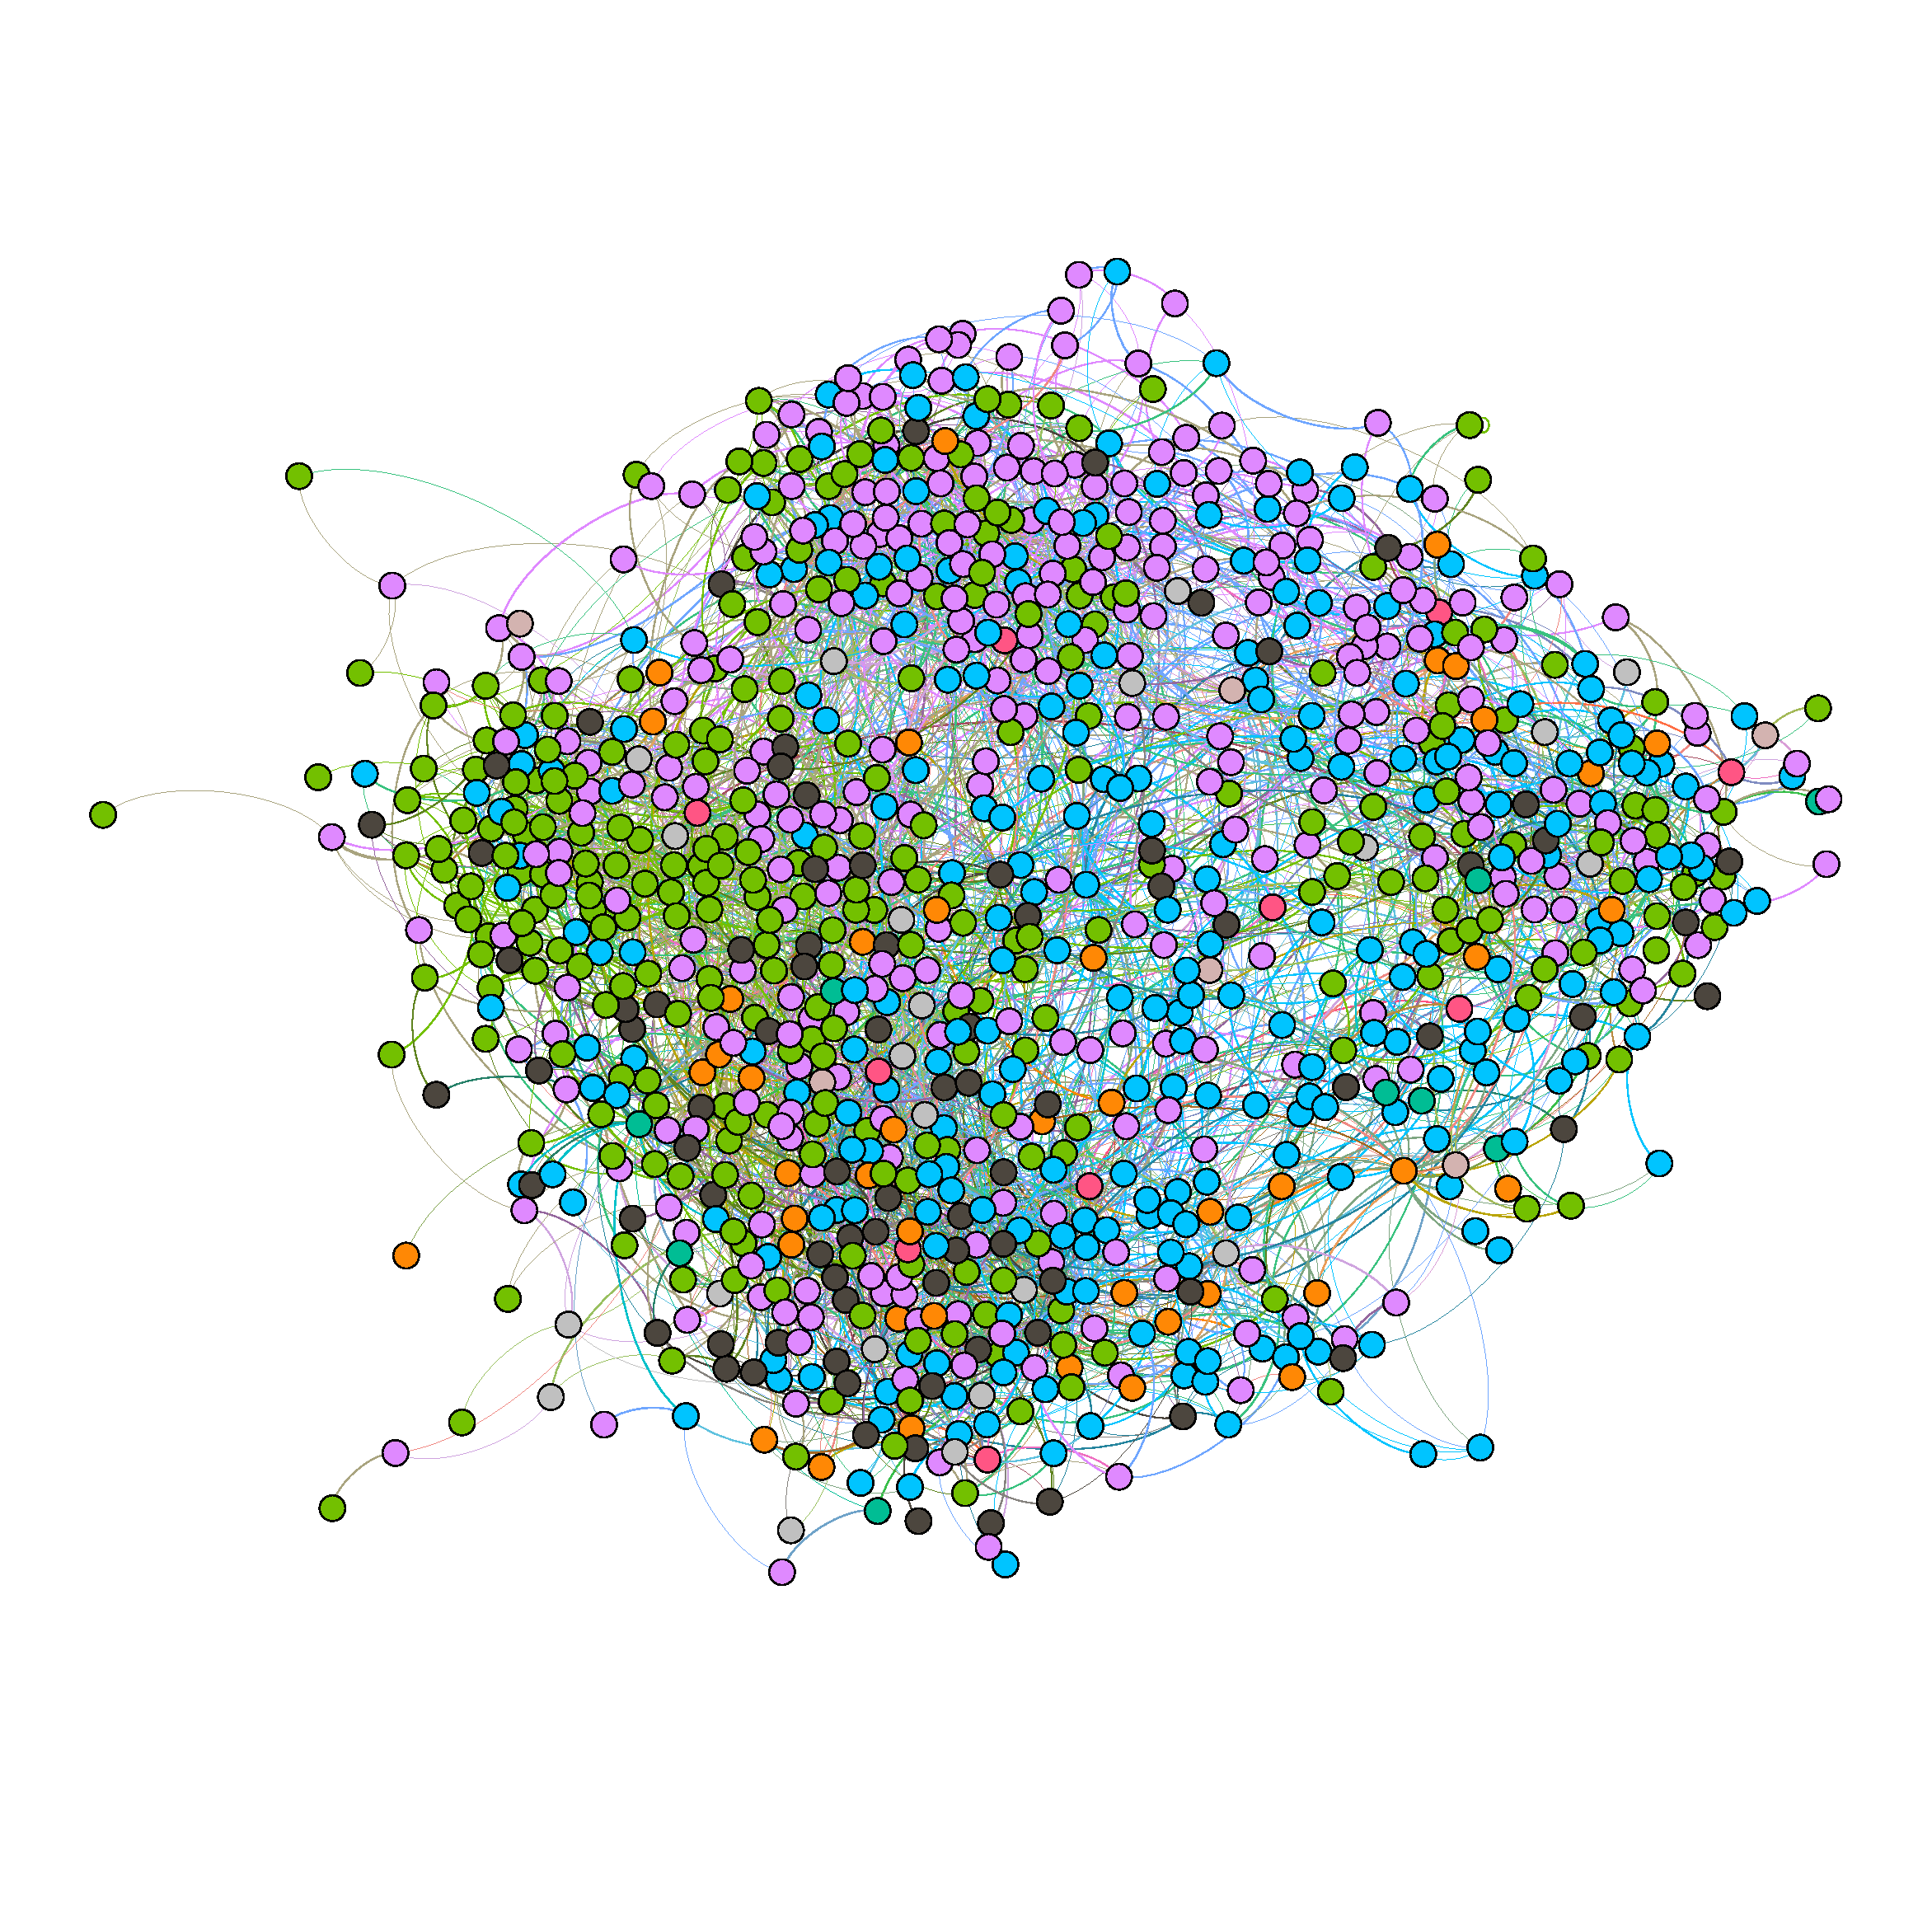
\includegraphics[width=\textwidth]{img/dim7_news.pdf}
    \label{fig:bubble5news}
    \caption{bubble3news}
  \end{subfigure}
  \caption{Simulations for 1000 users and 20 sources after 1000
    iterations. (\ref{fig:bubble3mod}), (\ref{fig:bubble5mod}) and
    (\ref{fig:bubble7mod}) highlights state vector.
    (\ref{fig:bubble3news}), (\ref{fig:bubble3news}) and
    (\ref{fig:bubble3news}) hightlitghts different news.
}
  \label{fig:test}
\end{figure}
